% !TEX root = ../Planning.tex
\section{Project description (D)}
\label{sec:project-description}

\subsection{The Ampersand project}
In November 2003, the Business Rules Manifesto\footnote{\url{http://www.businessrulesgroup.org/brmanifesto.htm}} was written, with the main purpose of declaring independence for business rules in the world of requirements.
The manifesto supports the vision of business rules as equivalent to requirements.
This is considered a radical change on how people see the world of business architecture.

In December 2010, Stef Joosten, Lex Wedemeijer and Gerard Michels published the paper ``Rule Based Design'', presenting the Ampersand approach.
The approach puts the rules in the center, using them to define the business processes.
Ampersand is named after the \& symbol with the desire of realizing results for both business and IT, in an efficient and effective way.

In 2011, the Ampersand compiler was created as an open source project.
Since then, the compiler has been improved and applied in both business and academic contexts.
The Ampersand end-users write business rules in a specific language (ADL), and compile that specification into functional specification, documentation and working software prototypes.
\dict{ADL}{Ampersand Design Language}%

The theory behind Ampersand has been throughly studied, and is based on mathe\-matical concepts, e.g. Tarski's axioms.
Using this compiler, users write the requirements in ADL and generate all the system specification.
This way the requirements consistency and traceability are always correct, from the lowest level up to the front-end.
The requirements can be presented to business stakeholders in natural language, guaranteeing that any business expert (who is knowledgeable in matters of content) can validate the requirements.

\subsection{Current situation}
The compiler developed for the Ampersand research project runs in several steps (see \autoref{subsec:architecture} for the architecture).
The first step is the parsing of the input scripts.
One of the main complaints from users is the quality of the errors generated by the Ampersand parser.
Since the beginning of the project, the parser subcomponent has never been analyzed for improvements.

In order to generate better error messages, it is assumed that a complete refactoring of the parser will be necessary.
The main challenge is to choose the correct kind of architecture and libraries in order to generate the most user-friendly messages possible.

Besides the main project task of improving the parser's feedback, a list of user wishes has accumulated over the years.

\subsection{Goals of the project}
The main objective for the graduation project is to implement useful feedback in the Ampersand parser.
In order to achieve this goal, some of the following activities can take place:
\begin{itemize}
	\item Analysis of user-friendly messages in compilers;
	\item Comparison of different Haskell parsing libraries (also for pretty-printing);
	\item Researching tools and techniques in Haskell for improving the software quality (e.g. testing and error messages);
	\item Analysis of the current development environment in relation with software engineering principles such as continuous delivery/integration;
	\item Recommending improvements for the overall software quality;
\end{itemize}
%
In case the new parser is successfully implemented and accepted, while the project members still have time budget available, the list of open user wishes issues can be addressed.
Some of these wishes are substantial, so that most of them cannot be fulfilled during the graduation project.
The current list of open issues has been provided\footnote{\url{https://github.com/AmpersandTarski/ampersand/tree/ABI\_Parser/ArchitectureAndDesign}}, although it must be clear that the issues are strictly seen as lower priority.

\subsection{Project architecture, components and environment}
\label{subsec:architecture}
The Ampersand compiler is divided in several subcomponents:
\dict{P-structure}{The parse-tree generated by the Ampersand parser, used as input for the type checker.}%
\dict{A-structure}{The ADL code generated by the Ampersand type checker, used as input for the calculator component.}%
\dict{ADL-structure}{See A-structure.}%
\dict{F-structure}{The functional structure generated by the Ampersand calculator, used as input for the different output modules.}%
\begin{description}
	\item[Parser] receives the ADL code as input, and parses that code into a parse-tree (also known as P-structure).
	\item[Type checker] receives the P-structure as input and converts it into a relation algebra format, suitable for manipulation (also known as A-structure or ADL-structure).
		 The semantics of ampersand are expressed in terms of the A-structure.
	\item[Calc] receives the A-structure as input, and manipulates it according to the research rules, generating the functional structure (also known as F-structure).
		The F-structure contains all design artifacts needed to write a specification and generate the output.
	\item[Output components]: All design artifacts present in the F-structure are ready to be rendered.
		Several components use this data structure to generate the wished output.
		Outputs currently implemented (and their output formats) are the following: Atlas (HTML interface), revert (Haskell source), Query (prototype generation) and Documentation Generator (Pandoc structure).
\end{description}
%
The complete architecture is depicted in \autoref{fig:architecture}.
The part of this architecture relevant for this project is depicted in \autoref{fig:data-flow}.
%
\begin{figure}[h]
	\centering
	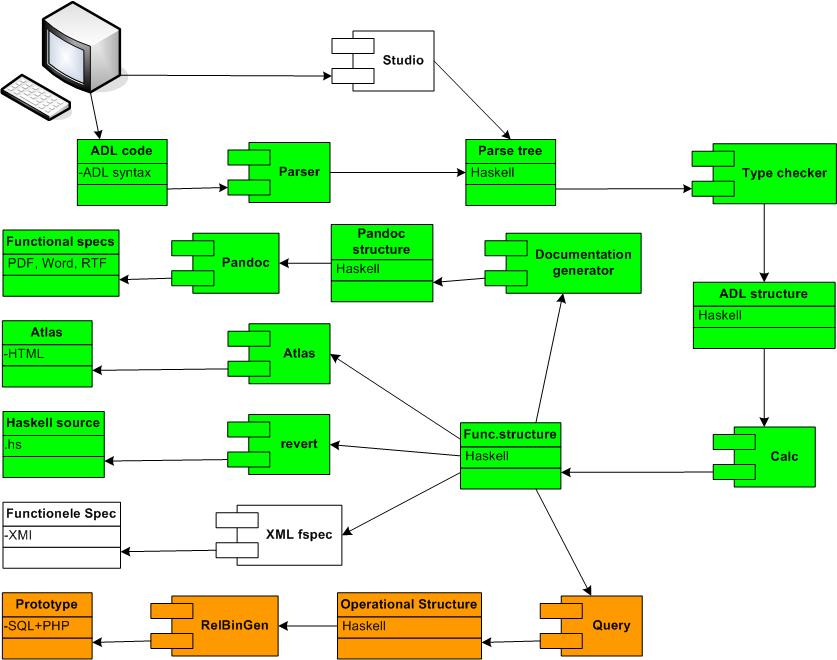
\includegraphics[width=\textwidth]{Figures/ADL_systeemarchitectuur}
	\caption[Architecture of the project]{Architecture of the project, showing where the parser fits in the Ampersand system}
	\label{fig:architecture}
	\small
	The components in green background are part of the Ampersand compiler.
	Components in orange are part of the Ampersand Prototype compiler.
	Finally, components in white background are future components, not yet implemented.
\end{figure}
%
\begin{figure}[h]
	\centering
	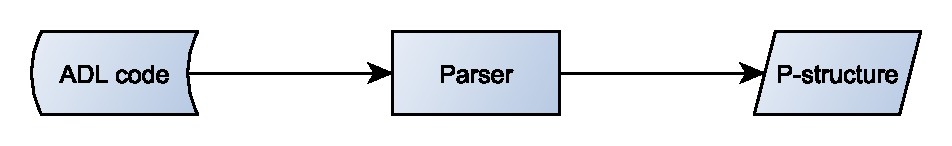
\includegraphics[width=0.5\textwidth]{Figures/Architecture}
	\caption{Relevant data flow for the Ampersand parsing component}
	\label{fig:data-flow}
\end{figure}

\subsection{Critical success factors}
The following factors are critical for the project's successful conclusion:
\begin{description}
	\item[Maintainability]: the code shall at least be as maintainable as the current Ampersand code.
		It is known however that maintainability is hard to measure (see also \autoref{sec:risk-management}).
	\item[Production code]: the implemented functionalities shall be integrated into the master branch for production use;
	\item[Users context]: in order to provide useful feedback, the user context wherein the Ampersand compiler is used needs to be well understood, and the improvements must have extra user value;
\end{description}

\subsection{Objectives and commitments}
Towards the project and customer
